\documentclass[paper=a4, fontsize=11pt]{article} % A4 paper and 11pt font size
%\usepackage[utf8x]{inputenc}
%\usepackage[czech]{babel} % English language/hyphenation
\usepackage{amsmath,amsfonts,amsthm} % Math packages
%\usepackage{lipsum} % Used for inserting dummy 'Lorem ipsum' text into the template
%\usepackage{sectsty} % Allows customizing section commands
%\allsectionsfont{\centering \normalfont\scshape} % Make all sections centered, the default font and small caps
\usepackage{fancyhdr} % Custom headers and footers
\pagestyle{fancyplain} % Makes all pages in the document conform to the custom headers and footers
\usepackage{graphicx}% For inserting images
\usepackage{wrapfig}% For wrapping images
\fancyhead{} % No page header - if you want one, create it in the same way as the footers below
\fancyfoot[L]{} % Empty left footer
\fancyfoot[C]{\thepage} % Empty center footer
\fancyfoot[R]{} % Page numbering for right footer
\renewcommand{\headrulewidth}{0pt} % Remove header underlines
\renewcommand{\footrulewidth}{0pt} % Remove footer underlines
\usepackage{graphicx}
\usepackage{indentfirst}
\usepackage[table]{xcolor}
\usepackage{booktabs}
\newcommand{\ra}[1]{\renewcommand{\arraystretch}{#1}}
\usepackage[
backend=biber, 
natbib=true,
style=numeric,
sorting=none
]{biblatex}
%\usepackage{hyperref}
\setlength\parindent{20pt} % Removes all indentation from paragraphs - comment this line for an assignment with lots of text
\usepackage{amssymb}
% Margins
\topmargin=-0.75in
\evensidemargin=0.0in
\oddsidemargin=-0.5in
\hoffset=1.0in
\textwidth=5.5in
\textheight=9.0in
\headsep=0.25in
%----------------------------------------------------------------------------------------
%	TITLE SECTION
%----------------------------------------------------------------------------------------

\newcommand{\horrule}[1]{\rule{\linewidth}{#1}} % Create horizontal rule command with 1 argument of height

%----------------------------------------------------------------------------------------
%	REFERENCES
\addbibresource{Report.bib}
%----------------------------------------------------------------------------------------

\title{	
\normalfont \normalsize 
\textsc{American University of Armenia} \\ [25pt] % Your university, school and/or department name(s)
\horrule{0.5pt} \\[0.4cm] % Thin top horizontal rule
\huge Applying various game search algorithms to Quarto\\ % The assignment title
\horrule{2pt} \\[0.5cm] % Thick bottom horizontal rule
}

\author{
	Petros Tepoyan \\
	Gogo Hovhannisyan \\
	Anna Abrahamyan } % Your name

\date{\normalsize\today} % Today's date or a custom date

\begin{document}

\maketitle % Print the title

\section*{Abstract}

Among many two-player games like “tic tac toe,” there also exists a game called Quarto. Quarto is a fun game played by two players. Before starting the game, a 4x4 grid is formed with 16 unique pieces and a player that succeeds in placing four pieces with the same property in a single line wins. In this project, we develop various search algorithms that analyze the state space of the game, using Minimax, Alpha-Beta and H-Minimax searches. We aim to show that the artificial intelligence heuristic approach gives an excellent performance for developing quarto strategies.

%\newpage

\tableofcontents

\newpage

\section{Introduction}


\begin{wrapfigure}{R}{0.25\textwidth}
	\centering
	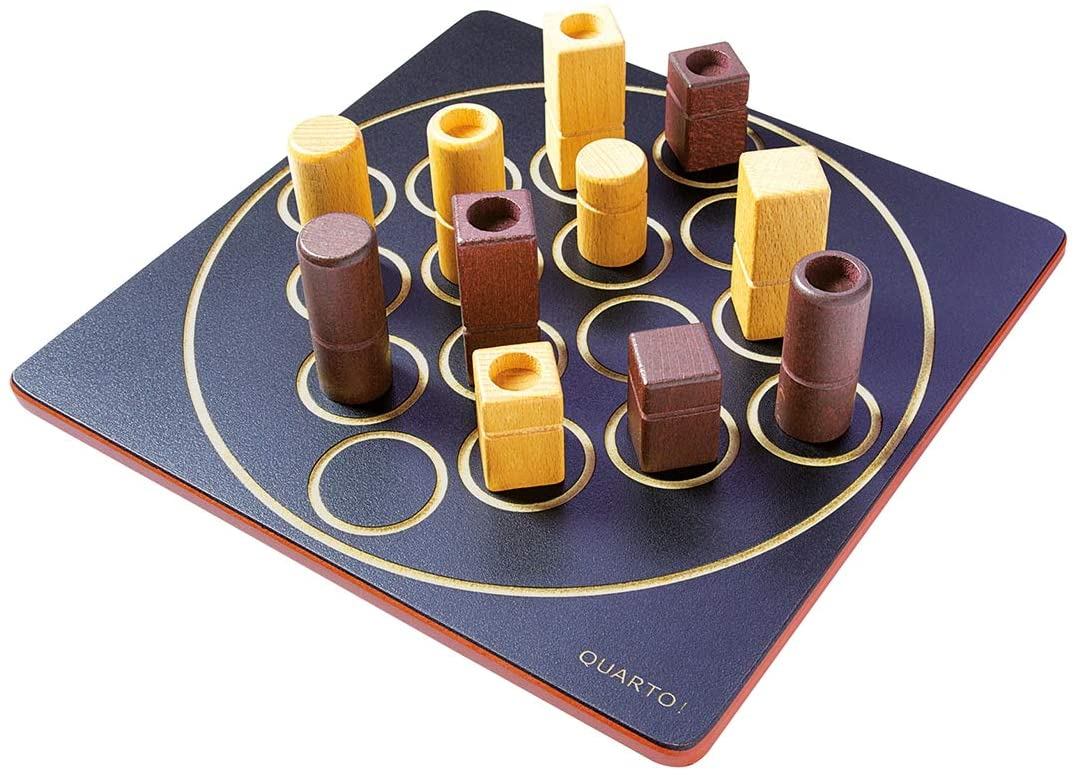
\includegraphics[width=0.25\textwidth]{quarto_game}
	\caption{Example of triples from \cite{cpluscode}}
\end{wrapfigure}

The quarto is a unique board game for two players invented by Swiss mathematician Blaise Muller. It has a 4x4 grid surrounded by a circle illustrated in Figure 1. The game is played in 16 pieces with different shapes. Each piece has four dichotomous attributes – color, height, shape, and consistency – so each piece is either black or white, tall or short, square or round, and with or without a hole. The object is to place the fourth piece in a row in which all four pieces have at least one attribute in common. 

The player who achieves this first is considered the winner. The twist is that the opponent gets to choose the piece another one places on the board each turn. In addition, quarto is a zero-sum game. A zero-sum game is a situation in which one person or group can win something only by causing another person or group to lose it.

Even though the Quarto game is not that popular and its community is relatively small compared to the other two-player games, it has exciting characteristics in developing an AI for Quarto. 


\section{Literature review}
As we already mentioned, the Quarto game community is small compared to other two-player games, and that is why there were very few reports and articles regarding the implementation of the Quarto game in AI. 
\subsection{AI for Quarto in Java}
In 2013, M. Neumann, J. Mohrmann, and D. Suendermann presented an artificial intelligence (AI) for the Quarto game in Java. During their project, they used minimax alpha-beta pruning to improve the runtime performance, depth-first search for decision making, and transposition table. As they mentioned in their report, there were no publications in relevant literature dealing with building an AI for the game Quarto up to 2013. \cite{AMohrmann2013}

A thorough review of the literature revealed the methods the authors used for their project. As mentioned in the report, after defining the PEAS, they used the alpha-beta pruning tree search algorithm to develop the AI. As their goal was to implement an AI with an acceptable time frame, the authors decided to implement a heuristic function, which will improve the performance of the AI.

‘In Quarto, the higher the number of lines that can be completed with a given piece (rows, columns, or diagonals), the higher the chance that one of these lines can be ultimately completed. So, depending on whose turn is to be evaluated, the heuristic function takes the number of such possible lines.’ \cite{AMohrmann2013}
According to the literature evidence base, there is an advantage while using the evaluation function, rather than implementing only the alpha-beta pruning algorithm. After completing the tasks and running their code multiple times, the authors figured that the Quarto AI was able to beat the clear majority of human players. ‘Overall, the ‘Quarto!’ AI won 34 out of 50 games.’ \cite{AMohrmann2013}

\subsection{Quarto using Alpha-Beta Pruning with two heuristics by C++}
Another interesting project was done again in 2013 by J. Bednarik, T. Dohnalek from the Norwegian University of Science and Technology. Their goal was to implement the game quarto using Alpha-Beta Pruning by C++ \cite{cpluscode}. 

The authors mentioned in the report that due to the computational difficulty, the agent isn’t able to explore the game states entirely. Hence they came up with two heuristic functions, improving both time and returning the value that describes the game state the best. The first heuristic function is checking in every move whether the piece the player chooses would not enable the opponent to win in the next move. Moreover, the second one is to examine the number of pieces the player can choose from so that he would not lose.

For having more accurate results, the authors implemented several different kinds of players such as Random, Novice, Minimax with different depths of search, Human player and also Remote player( other application). They played games with different pairs of their players, and the results showed that Novice was better than Random, Minimax-3 played better than Novice, and lastly, Minimax-4 won more than Minimax-3.

According to this literature evidence base and their results after playing the game with other applications, it was noticeable that the implemented Minimax player was able to easily beat all other opponents, including some applications the authors have explored on the Internet. 
\subsection{Multi-Agent AI for Quarto by HTTP Requests}
Moreover, in 2015 Grant Jenks created a project, which again developed an AI for Quarto \cite{QuartoJenks}. Their goal was to create computer players that could play the game Quarto with each other. They use one recursive Minimax algorithm for solving the Quarto game, however instead of a move computing heuristic function, they track to win, draw, lose, unknown and out-of-time states. The algorithm does an iteratively increasing depth-limit search for the best solution. Their program is a multiagent version of the Quarto game, as another server sends an HTTP request asking a specific player to join a session. Furthermore, all the next moves are made by sending requests to each other by HTTP. They wanted to implement a code with the highest performance, and they succeeded. 

\subsection{Planning the Quarto game for AI Development}
In 2017, Julien Mattiussi, a full-stack web developer at Marmelab, presented another project, which was later posted in Github in 2019 by Alexis Janvier \cite{Mattiussi2018}. Their project was to create an AI for Quarto, and they presented the planning of how their code works. 
It was challenging to understand how the code works, as the report was in French, but we managed to understand the idea of their project. In their program, the authors defined the game board and actions; they mainly concentrated on the graphic interpretation of the program, then defined the current state using python language. They created 16 pieces with their four characteristics. Moreover, the winner will be by comparing their common characteristics using the binary and logical operators. Their approach was very interesting and easy. 

\subsection{Conclusion}
Although the game Quarto is not very famous, it still represents a thought-provoking aspect and so therefore it is a good idea to develop an AI algorithm to perform well in the game. It makes players think in 4 directions simultaneously, as in order to make a smart move, they need to consider 4 characteristics of the pieces. It will only influence players to play the game at the top level. After understanding how the AI works, how it finds the best solutions in a very limited time, players can utilize the AI game logic to analyze both their and their opponent’s games better. 
The goal of this literature review was to compare the existing projects about the Quarto AI game and understand what techniques and methods we can implement to get a better version of the game. The reviewed literature suggests that there are advantages to the use of state evaluation functions because they will only improve the minimax algorithm by choosing the best solution in different states. 


\section{Methods} \label{txt:tech}
To start our discussion, we need to define the architecture of our implementation. Section 3.2 describes the hierarchy of the modules, and sections 3.3, 3.4 introduce the contents of the modules themselves. 

\subsection{Chosen technologies}
We are going to use the programming language Python, as it has a very solid and flexible base for OOP. For faster work with arrays, we will use \verb|numpy| library.

\subsection{Modules architecture}
Below are described the modules of our OOP solution. Abstract classes are in \textit{italics}, inheritance is in round brackets.
\begin{itemize}
	\item[$\blacksquare$] piece
	\begin{itemize}
		\item[$\circ$] Piece
	\end{itemize}

	\item[$\blacksquare$] turn
	\begin{itemize}
		\item[$\circ$] \textit{Action}
		\item[$\circ$] Turn(Action)
	\end{itemize}

	\item[$\blacksquare$] board
	\begin{itemize}
		\item[$\circ$] \textit{State}
		\item[$\circ$] Board(State)
		\item[$\circ$] \textit{TerminalTest}
		\item[$\circ$] BoardTerminalTest(TerminalTest)
	\end{itemize}

	\item[$\blacksquare$] player
	\begin{itemize}
		\item[$\circ$] Player
	\end{itemize}

	\item[$\blacksquare$] search
	\begin{itemize}
		\item[$\circ$] \textit{Search}
		\item[$\circ$] MinimaxSearch(Search)
		\item[$\circ$] AlphaBetaSearch(Search)
		\item[$\circ$] HeuristicMinimaxSearch(Search)
	\end{itemize}
	\item tools
\end{itemize}

\subsection{Game formation}

Module \verb|piece| contains a single class with the same name, that represents a playing piece, which can be white or black, round or square, big or small, and having a hole or not. Module \verb|turn| contains a class \verb|Turn|, which encapsulates the notion of a game turn; it contains information about the current player, what piece that player has to place, coordinate of that placed piece (if placed), and the previous turn (if present). Module \verb|board| contains two classes \verb|Board| and \verb|BoardTerminalTest|. The class \verb|Board| contains information about a state of the game, such as game turn, grid, and the remaining pieces. It also has methods to return all applicable actions given its properties and result of those actions. The class \verb|BoardTerminalTest| contains methods for evaluting if it is a terminal state and what is its utility value.

A tricky part about the implementation is that a turn is not really the turn we mean when we say that word, since it is comprised of receiving a figure, placing it, and choosing a new one. Hence, we define a turn as follows. If there is a piece to place (that is given in \verb|Turn| object), the player has to place that piece and choose another one. In a nutshell, a turn is: place (if applicable) a piece and choose a new piece for the opponent. A player may not have a piece to place only in two cases: if it is the very first turn, as one player has to choose one figure for its opponent to start the game; if it is the very last turn, which will result in termination.

\subsection{Search formation}

Talking about the implementation of the search algorithms, we can start from describing basic capabilities of an abstract class \verb|Search| in the module \verb|search|. The mail responsibilities are to find and return a strategy to a problem and return a number of generated states. The classes \verb|MinimaxSearch|, \verb|AlphaBetaSearch| and \verb|HeuristicAlphaBetaSearch| perform the searches of the same names. Furthermore, when initializing a search, we can specify a flag \verb|optimized|. If set to \verb|True|, the algorithm will first check if there is already a utility value for a state, and if there is one, return it immediately. In other words, we will exclude state repetition. 


\subsubsection{Search algorithms} 
\begin{enumerate}
	\item 
	The Minimax algorithm is the most well-known two-player, zero-sum game strategy. Minimax is a technique for limiting the largest probable loss that can occur as a result of a player’s decision. The Maximax concept advises players to select the approach that produces the best of all potential outcomes \cite{StrToPlay}.
	
	\item 
	The heuristic approach is very similar to minimax but is much better in terms of time complexity. A heuristic is a way of problem-solving that uses a practical method or a series of shortcuts to provide solutions that are not perfect but are adequate given a limited period or deadline \cite{Heu}.
	
	\item
	Alpha-beta pruning is a modified version of the minimax algorithm. It is a significant enhancement to the minimax search algorithm that eliminates the need to search large portions of the game tree using a branch-and-bound technique. Alpha and beta represent the minimum score that the maximizing player is assured of and the maximum score that the minimizing player is assured of, respectively \cite{AB}.
\end{enumerate}

\subsubsection{State evaluation function} 
For the heuristic approach, we will need state evalution functions. In our case, we suggest the \textbf{number of non-terminal pieces}. 

\begin{wrapfigure}{R}{0.25\textwidth}
	\centering
	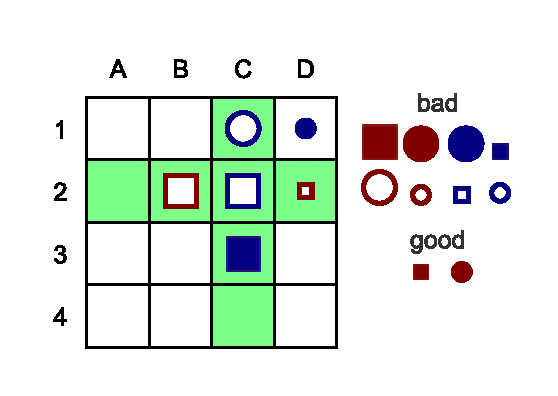
\includegraphics[width=0.25\textwidth]{heuristic_function}
	\caption{Example of triples from \cite{cpluscode}}
\end{wrapfigure}

During the game, the players will arrange their pieces in a way that there will be triples - sequence of three pieces with the same property in a line - which need one right piece to terminate the game \cite{cpluscode}.

 If there are is white triplet and it is the turn of Bob to select a piece for Alice, he should not select a white piece, as Alice will complete the triplet and win. Similarly, if there is another triple, three small pieces, and it is the turn of Alice, she should not give small ones as well; hence, she should filter out white and small ones. The count number of the resulting pieces is exactly the value of this heuristic function.
 
\section{Plan} \label{txt:arch}
What is left for us at this point is to finalize the code, and start testing. Since we have the real game with us, we can test AI based agent against any of us. Later on we will add a section where we discuss our findings and a link to the github repository with all the materials we used for this project.

\printbibliography
%-----------------------------------------------
\begin{flushleft}
%\bibliography{literatura} % viz. literatura.bib..
%\bibliographystyle{czplain}
\end{flushleft}
\end{document}
